\documentclass{article}
\usepackage{amssymb} % Required for math symbols
\usepackage{graphicx} % Required for inserting images

\usepackage[utf8]{inputenc}
\usepackage{amsmath}
\usepackage[a4paper, total={7in, 10in}]{geometry}

\title{Poisson Blending}
\author{jeremy.matos}
\date{June 2024}

\begin{document}

\maketitle

\section{Introduction}

The mathematical tool at the heart of the approach is the Poisson partial differential equation with Dirichlet boundary conditions which specifies the Laplacian of an unknown function over the domain of interest, along with the unknown function values over the boundary of the domain. The motivation is twofold.

\subsection*{Poisson partial differential equations}

\subsection*{Dirichlet boundary conditions}

\subsection*{Laplacian operator}

\section{Poisson solution to guided interpolation}

\subsection*{Guided interpolation}

\begin{itemize}
    \item Image interpolation using a guidance vector field
    \item Solve the interpolation problem for each color component separately
\end{itemize}

\begin{itemize}
    \item Let $S$ a closed subset of $\mathbb{R}^2$, be the image definition domain.    % target total image
    \item Let $\Omega$ be a closed subset of $S$ with boundary $\partial \Omega$.   % target mask image
    \item Let $f*$ be a known scalar function defined over $S$ minus the interior of $\Omega$.   % total_target - target_mask_image
    \item Let $f$ be a unknown scalar function defined over the interior of $\Omega$.   % source image to blend
    \item Let $v$ be a vector field defined over $\Omega$ 
\end{itemize}

\begin{figure}[h!]
    \centering
    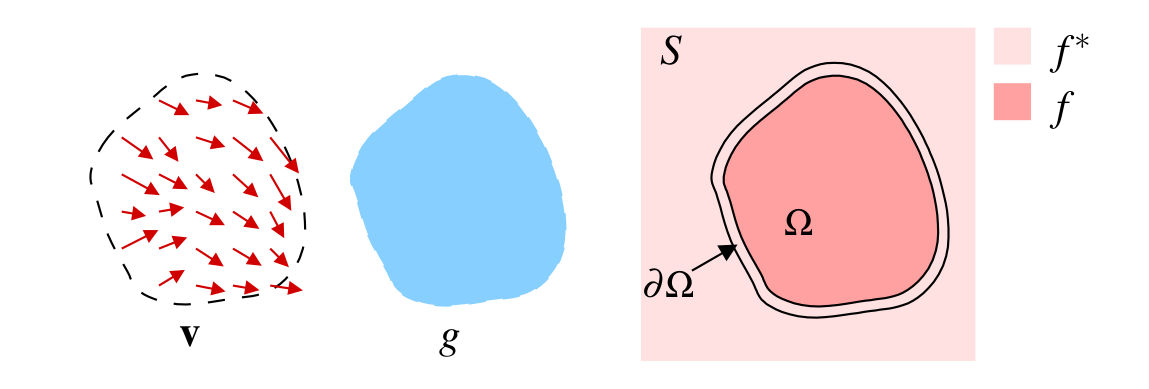
\includegraphics[width=0.7\textwidth]{figure_1.png}
    \caption{Guided interpolation notations. Unknown function $f$ interpolates in domain $\Omega$ the destination function $f^*$, under guidance of vector field $v$, which might be or not the gradient field of a source function $g$.}
    \label{fig:guided_interpolation}
\end{figure}

The simplest interpolant $f$ of $f*$ over $\Omega$ is the membrane interpolant defined as the solution of the minimization problem:

\begin{equation}
    \min_f \iint_\Omega |\nabla f|^2 \ \text{with} \ f|_{\partial \Omega} = f^*|_{\partial \Omega}
\end{equation}

% "Minimizar respecto a $f$ la integral doble sobre el dominio $\Omega$ de la norma del gradiente de $f$ al cuadrado, con la condición de que $f$ en el borde de $\Omega$ sea igual a $f*$ en el borde de $\Omega$."

where $\nabla . = (\frac{\partial_.}{\partial_x}, \frac{\partial_.}{\partial_y})$ is the gradient operator. The minimizer must satisfy the associated Euler-Lagrange equation:

\begin{equation}
    \Delta f = 0 \ \text{over} \ \Omega \ \text{with} \ f|_{\partial \Omega} = f^*|_{\partial \Omega}
\end{equation}


where $\Delta . = (\frac{\partial^2_.}{\partial_{x^2}}, \frac{\partial^2_.}{\partial_{y^2}})$ is the Laplacian operator. Equation 2 is a Laplace equation with Dirichlet boundary conditions.

The route proposed in this work is to modify the problem by introducing further constraints in the form of a guidance field as follows:

A \textbf{guidance field} is a vector field $\mathbf{v}$ used in an extended version of the minimization problem (1) above:

\begin{equation}
    \min_f \iint_\Omega |\nabla f - \mathbf{v}|^2 \ \text{with} \ f|_{\partial \Omega} = f^*|_{\partial \Omega}
\end{equation}

whose solution is the unique solution of the following Poisson equation with Dirichlet boundary conditions:

\begin{equation}
    \Delta f = \text{div}\mathbf{v} \ \text{over} \ \Omega \ \text{with} \ f|_{\partial \Omega} = f^*|_{\partial \Omega}
\end{equation}

where $\text{div} . = \frac{\partial_.}{\partial_x} + \frac{\partial_.}{\partial_y}$ is the divergence operator of $\mathbf{v} = (u, v)$. 

Three Poisson equations of the form (4) are solved independently in the three color channels of the chosen color space.


When the guidance field $\mathbf{v}$ is conservative, i.e., it is the gradient of some function $g$, a helpful alternative way of understanding what Poisson interpolation does is to define the correction function $\tilde{f}$ on $\Omega$ such that $f = \tilde{f} + g$. The Poisson equation (4) then becomes:

\begin{equation}
    \Delta \tilde{f} = 0 \ \text{over} \ \Omega \ \text{with} \ \tilde{f}|_{\partial \Omega} = (f^* - g) |_ {\partial \Omega}
\end{equation}

\subsection*{Discrete Poisson solver}

\subsection*{Seamless cloning}

\end{document}

% https://tug.ctan.org/info/undergradmath/undergradmath.pdf